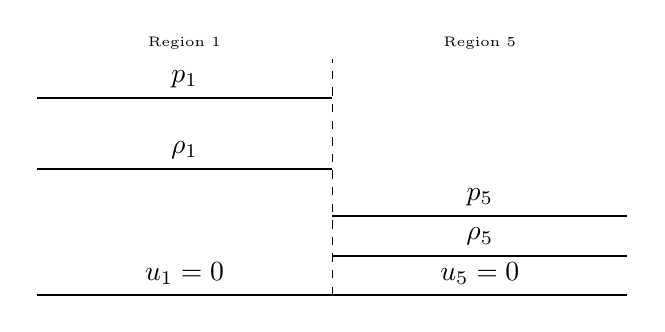
\begin{tikzpicture}
		%ground nodes
	\node [] at (0,0) (a0) {};
	\node [] at (3.75,0) (a3) {};
	\node [] at (7.5,0) (a6) {};
		%level 1 nodes
	\node [] at (0,1.6) (f0) {};
	\node [] at (3.75,1.6) (f1) {};
	\node [] at (7.5,0.5) (b6) {};
	
		%level 2 nodes
	\node [] at (0,2.5) (h0) {};
	\node [] at (3.75,2.5) (h1) {};
	\node [] at (3.75,0.5) (b3) {};
	\node [] at (7.5,1) (d6) {};
	\node [] at (3.75,1) (d3) {};	
		%top nodes
	\node [] at (0,3) (i0) {};
	\node [] at (3.75,3) (i3) {};
	\node [] at (7.5,3) (i6) {};
	
	\draw[thick] (a0.center) -- (a3.center) node [midway,above] {$u_1=0$};
	\draw[thick] (f0.center) -- (f1.center) node [midway,above] {$\rho_1$};
	\draw[thick] (h0.center) -- (h1.center) node [midway,above] {$p_1$};
	
	\draw[thick] (a3.center) -- (a6.center) node [midway,above] { $u_5=0$};
	\draw[thick] (b3.center) -- (b6.center) node [midway,above] {$\rho_5$};
	\draw[thick] (d3.center) -- (d6.center) node [midway,above] {$p_5$};
	\draw[dashed] (a3.center) -- (i3.center) {};
	\path[] (i0.center) -- (i3.center) node [midway,above] {\tiny Region 1};
	\path[] (i3.center) -- (i6.center) node [midway,above] {\tiny Region 5};
\end{tikzpicture}